\begin{mybilan}
	
	\twoCol{
	\begin{center}
		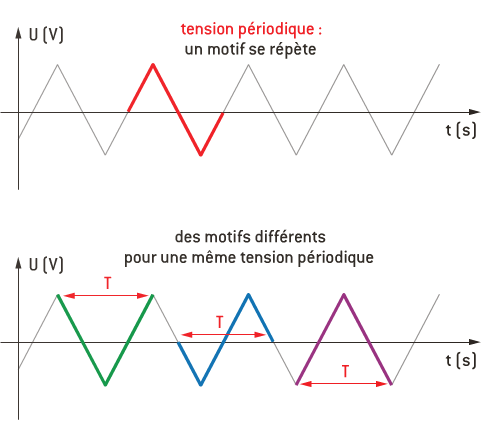
\includegraphics[scale=0.7]{bilan3}
	\end{center}

	\begin{itemize}
		\item Une tension est \kw{périodique} lorsque ses \kw{variations se répètent} identiques à elles mêmes au cours du temps. 
		\item La \kw{durée} d'un motif est la \kw{période}. On la note $T$, son unité est la seconde $s$.
	\end{itemize}
	}

\end{mybilan}